\begin{question}
Design each of the following codes, and then calculate its average coding length, and
redundancy, per symbol.
\begin{enumerate}
\item A minimum variance Huffman code for the alphabet \{A, B, C, D\}, with probabilities, 0.1, 0.2, 0.3, \& 0.4, respectively.
\item A minimum variance extended Huffman code for the binary alphabet {0, 1}, with
probabilities 0.1 and 0.9, respectively. Generate a code word for every block of 3 symbol.
\item A 3-bit Tunstall code for the above binary alphabet.
\end{enumerate}
\end{question}
\begin{solution}

\begin{tabular}{||c|c||c|c||c|c||c|c||}
\hline 
\multicolumn{2}{||c||}{Min-Var Huffman} & \multicolumn{2}{||c||}{Huffman} & \multicolumn{2}{||c||}{Extended Huffman} & \multicolumn{2}{||c||}{Tunstall} \\ 
\hline 
Symbol & Code & Symbol & Code & Symbol & Code & Symbol & Code \\ 
\hline 
A & 011 & A & 001 & 000 & 11111 & 0 & 000 \\ 
\hline 
B & 010 & B & 000 & 001 & 11110 & 10 & 001 \\ 
\hline 
C & 00 & C & 01 & 010 & 11101 & 110 & 010 \\ 
\hline 
D & 1 & D & 1 & 011 & 11100 & 1110 & 011 \\ 
\hline 
• & • & • & • & 100 & 110 & 11110 & 100 \\ 
\hline 
• & • & • & • & 101 & 101 & 111110 & 101 \\ 
\hline 
• & • & • & • & 110 & 100 & 1111110 & 110 \\ 
\hline 
• & • & • & • & 111 & 0 & 1111111 & 111 \\ 
\hline 
$L_{ave}$ & 1.9  & $L_{ave}$ & 1.9  & $L_{ave}$ & 0.53 & $L_{ave}$ & 0.86  \\ 
\hline 
Red & 0.06 & Red & 0.06 & Red & 0.07 & Red & 0.4  \\ 
\hline 

\end{tabular} 

\end{solution}

\begin{question}
An alphabet is composed of the 6 symbols \{A, C, N, T, Y, $\Delta$\}. Design a minimum length code for the alphabet. Assign short codes for small index symbols. Use this code as a starting code during next problems.
\end{question}

\begin{solution}
\begin{tikzpicture}[level 1/.style={sibling distance=4cm},level 2/.style={sibling distance=2.5cm},level 3/.style={sibling distance=1cm}]
	\node {Root}
		child { node {0}
            child {node{0} 
                child{ node{0(A)}} 
                child{ node{1(C)}}}
			child {node{1}
			    child{ node{0(N)}} 
                child{ node{1(T)}}}		
		}
		child { node {1}
		    child{ node{0(Y)}} 
            child{ node{1($\Delta$)}}}		 		
	;
\end{tikzpicture}

\begin{tabular}{|c|c|}
\hline 
Symbol & Code \\ 
\hline 
A & 000 \\ 
\hline 
C & 001 \\ 
\hline 
N & 010 \\ 
\hline 
T & 011 \\ 
\hline 
Y & 10 \\ 
\hline 
$\Delta$ & 11 \\ 
\hline 
\end{tabular} 
\end{solution}

\begin{question}
Using adaptive Huffman coding,
\begin{enumerate}
\item code the following: “ACACTAN”. Show the development of the coding tree, and the code generated for each symbol.
\item Decode the first 5 symbols of the same alphabet, form the stream
“0111011001011001101100001111011000101001100011010101”
\end{enumerate}
\end{question}
\begin{solution}
\begin{enumerate}
\item Alphabet = \{A,C,N,T,Y,$\Delta$\} \\
$6=2^e + r$ \\
$e=2$ \\
$r=2$ \\
$\text{\#nodes}= 11$ \\
Initial codes: \\
\begin{tabular}{|c|c|}
\hline 
Symbol & Code \\ 
\hline 
A & 000 \\ 
\hline 
C & 001 \\ 
\hline 
N & 010 \\ 
\hline 
T & 011 \\ 
\hline 
Y & 10 \\ 
\hline 
$\Delta$ & 11 \\ 
\hline 
\end{tabular} 

\begin{itemize}
\item Code A = Code(NYT):Code(A). Transmit 000. \\
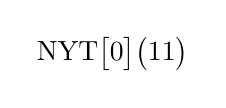
\begin{tikzpicture}[level 1/.style={sibling distance=4cm},level 2/.style={sibling distance=2.5cm},level 3/.style={sibling distance=1cm}]
	\node {NYT\big[0\big]\big(11\big)}		 		
	;
\end{tikzpicture}


\item Code C = Code(NYT):Code(C). Transmit 0001. \\
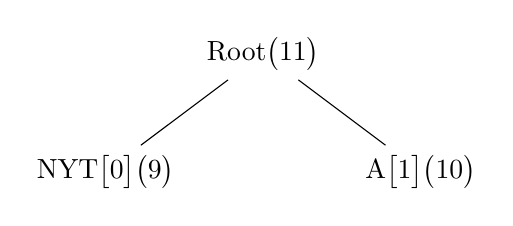
\begin{tikzpicture}[level 1/.style={sibling distance=4cm},level 2/.style={sibling distance=2.5cm},level 3/.style={sibling distance=1cm}]
	\node {Root\big(11\big)}
		child { node {NYT\big[0\big]\big(9\big)}}
        child { node {A\big[1\big]\big(10\big)}}	 		
	;
\end{tikzpicture}
\item Code A = 1. Transmit 1. \\
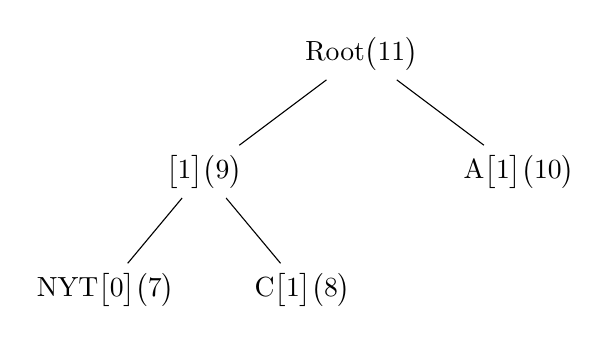
\begin{tikzpicture}[level 1/.style={sibling distance=4cm},level 2/.style={sibling distance=2.5cm},level 3/.style={sibling distance=1cm}]
	\node {Root\big(11\big)}
		child { node {\big[1\big]\big(9\big)} 
                child{ node{NYT\big[0\big]\big(7\big)}} 
                child{ node{C\big[1\big]\big(8\big)}}}
		child {node{A\big[1\big]\big(10\big)}}	
	;
\end{tikzpicture}
\item Code C = 01. Transmit 01. \\
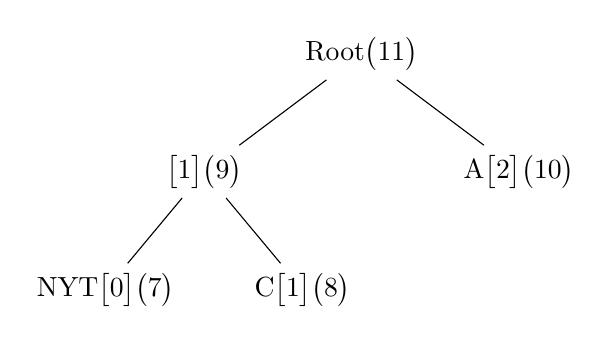
\begin{tikzpicture}[level 1/.style={sibling distance=4cm},level 2/.style={sibling distance=2.5cm},level 3/.style={sibling distance=1cm}]
	\node {Root\big(11\big)}
		child { node {\big[1\big]\big(9\big)} 
                child{ node{NYT\big[0\big]\big(7\big)}} 
                child{ node{C\big[1\big]\big(8\big)}}}
		child {node{A\big[2\big]\big(10\big)}}	
	;
\end{tikzpicture}
\item Code T = Code(NYT):Code(T). Transmit 00011. \\
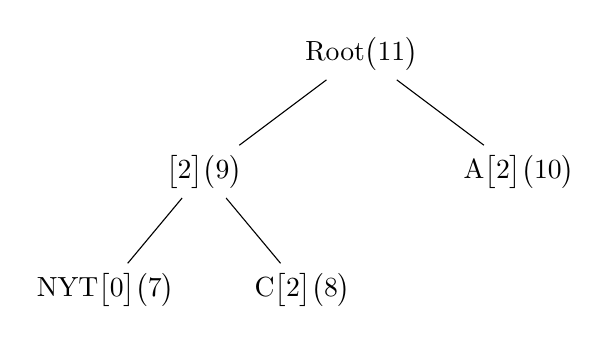
\begin{tikzpicture}[level 1/.style={sibling distance=4cm},level 2/.style={sibling distance=2.5cm},level 3/.style={sibling distance=1cm}]
	\node {Root\big(11\big)}
		child { node {\big[2\big]\big(9\big)}  
                child{ node{NYT\big[0\big]\big(7\big)}} 
                child{ node{C\big[2\big]\big(8\big)}}}
        child {node{A\big[2\big]\big(10\big)}}	
	;
\end{tikzpicture}
\item Code A = 1. Transmit 1. \\
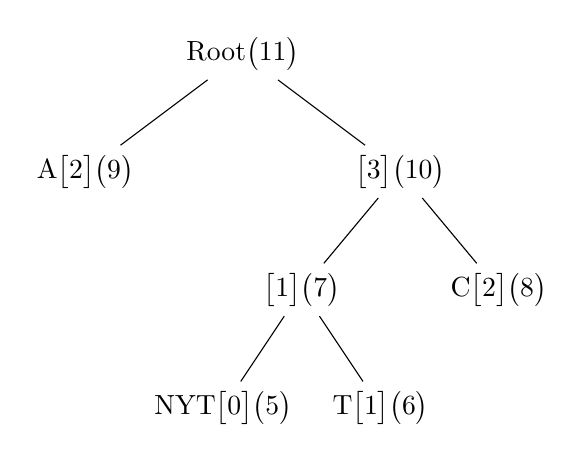
\begin{tikzpicture}[level 1/.style={sibling distance=4cm},level 2/.style={sibling distance=2.5cm},level 3/.style={sibling distance=2cm}]
	\node {Root\big(11\big)}
		child {node{A\big[2\big]\big(9\big)}}	
		child { node {\big[3\big]\big(10\big)}  
                child{ node{\big[1\big]\big(7\big)}
                        child{ node{NYT\big[0\big]\big(5\big)}} 
                        child{ node{T\big[1\big]\big(6\big)}}
                     } 
                child{ node{C\big[2\big]\big(8\big)}}
              }
               
	;
\end{tikzpicture}
\item Code N = Code(NYT):Code(N). Transmit 1000010.\\
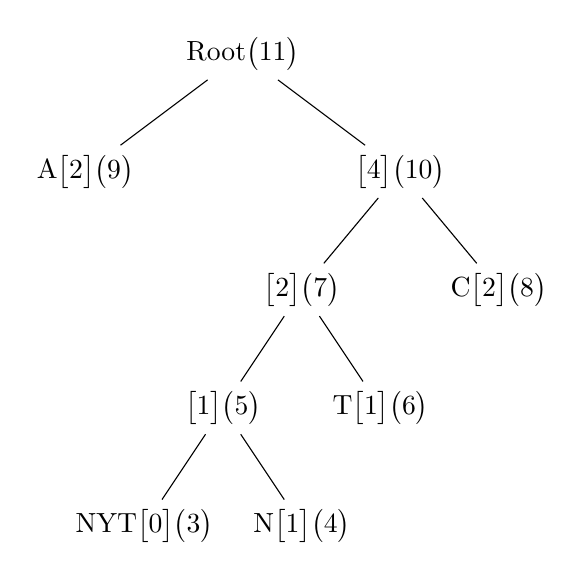
\begin{tikzpicture}[level 1/.style={sibling distance=4cm},level 2/.style={sibling distance=2.5cm},level 3/.style={sibling distance=2cm}]
	\node {Root\big(11\big)}
		child {node{A\big[2\big]\big(9\big)}}	
		child { node {\big[4\big]\big(10\big)}  
                child{ node{\big[2\big]\big(7\big)}
                        child{ node{\big[1\big]\big(5\big)} 
                                child{  node{NYT\big[0\big]\big(3\big)}}
                                child{  node{N\big[1\big]\big(4\big)}}
                             } 
                        child{ node{T\big[1\big]\big(6\big)}}
                     } 
                child{ node{C\big[2\big]\big(8\big)}}
              }
               
	;
\end{tikzpicture}
\end{itemize}
\item Decode “0111011001011001101100001111011000101001100011010101”.
\begin{itemize}
\item Encode 011 = T, then encode 1 = T, then encode 011=NYT+$\Delta$. \\
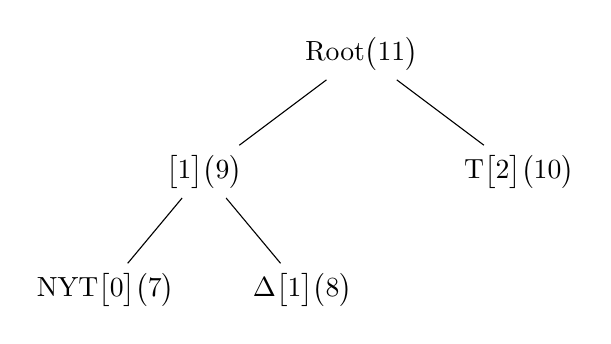
\begin{tikzpicture}[level 1/.style={sibling distance=4cm},level 2/.style={sibling distance=2.5cm},level 3/.style={sibling distance=2cm}]
	\node {Root\big(11\big)}
		child { node {\big[1\big]\big(9\big)}  
                child{ node{NYT\big[0\big]\big(7\big)}}
                child{ node{$\Delta$\big[1\big]\big(8\big)}}
              }
         child {node{T\big[2\big]\big(10\big)}}	
	;
\end{tikzpicture}
\item Encode 0010 = NYT+Y. \\
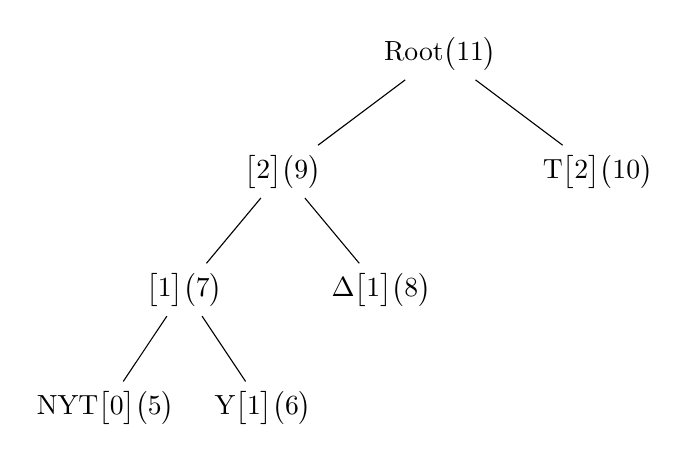
\begin{tikzpicture}[level 1/.style={sibling distance=4cm},level 2/.style={sibling distance=2.5cm},level 3/.style={sibling distance=2cm}]
	\node {Root\big(11\big)}
		child { node {\big[2\big]\big(9\big)}  
                child { node {\big[1\big]\big(7\big)}  
                            child{ node{NYT\big[0\big]\big(5\big)}}
                            child{ node{Y\big[1\big]\big(6\big)}}
                      }
                child{ node{$\Delta$\big[1\big]\big(8\big)}}
              }
         child {node{T\big[2\big]\big(10\big)}}	
	;
\end{tikzpicture}
\item Encode 1 = T.
\end{itemize}
$\therefore \text{final message}= T T \Delta Y T$.
\end{enumerate}
\end{solution}

\begin{question}
Use the Golomb code, with m=2, to code the above sequence.
\end{question}
\begin{solution}
\begin{tabular}{|c|c|c|c|c|c|c|c|c|}
\hline 
Symbol & A & C & A & C & T & A & N \\ 
\hline 
Code & 01 & 100 & 01 & 100 & 1100 & 01 & 101 \\ 
\hline 
\end{tabular} 
\end{solution}

\begin{question}
Code the above sequence using Move-To-Front.
\end{question}
\begin{solution}
\begin{tabular}{|c|c|c|c|c|c|c|c|c|}
\hline 
Symbol & A & C & A & C & T & A & N \\ 
\hline 
Code & 01 & 100 & 100 & 100 & 1100 & 101 & 1100 \\ 
\hline 
\end{tabular} 
\end{solution}

\begin{question}
Code the number 7 using.
\begin{enumerate}
\item Golomb code, with m=3.
\item Rice code, fundamental sequence.
\item Rice code, split sample option, with m=3, and k=5.
\end{enumerate}
\end{question}
\begin{solution}
\begin{enumerate}
\item 11010
\item 11111110
\item 1110
\end{enumerate}
\end{solution}

\begin{question}
Code the number 6. First, use Golomb code with m=3.
Next use Recursive indexing, with a
representation alphabet of size 3. Use variable
length code for entropy coding, with smaller
numbers having short length. Draw the VLC tree.
Label different parts of each code.

\end{question}
\begin{solution}
\begin{itemize}
\item Golomb code. q=2, r=0. Code = unary(2):prefix(0) = 1100
\item RI code. C(6)=$b_2b_2b_2b_0=00010$
\begin{tikzpicture}[level 1/.style={sibling distance=4cm},level 2/.style={sibling distance=2.5cm},level 3/.style={sibling distance=2cm}]
	\node {Root}
	    child {node{$b_2$}}	
		child { node {}  
                child{ node {$b_0$}}
                child{ node {$b_1$}}
              }
	;
\end{tikzpicture}

\end{itemize}
\end{solution}


\begin{question}
Using adaptive Huffman coding, code the string “COCOAC”. Show the development of the
coding tree. Assume that the used alphabet has only the 3 characters A, C, and O. Use VLC for new character coding.
\end{question}
\begin{solution}
Initial codes: \\
\begin{tabular}{|c|c|}
\hline 
A & 0 \\ 
\hline 
C & 10 \\ 
\hline 
O & 11 \\ 
\hline 
\end{tabular} \\

\begin{itemize}
\item Code C = 10. Transmit 10. \\
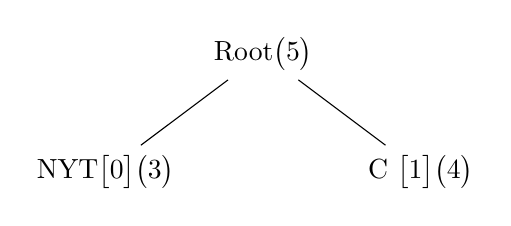
\begin{tikzpicture}[level 1/.style={sibling distance=4cm},level 2/.style={sibling distance=2.5cm},level 3/.style={sibling distance=2cm}]
	\node {Root\big(5\big)}
	    child { node{NYT\big[0\big]\big(3\big)}}	
		child { node{C  \big[1\big]\big(4\big)}}
	;
\end{tikzpicture} 
\item Code O = Code(NYT):Code(O). Transmit 011. \\
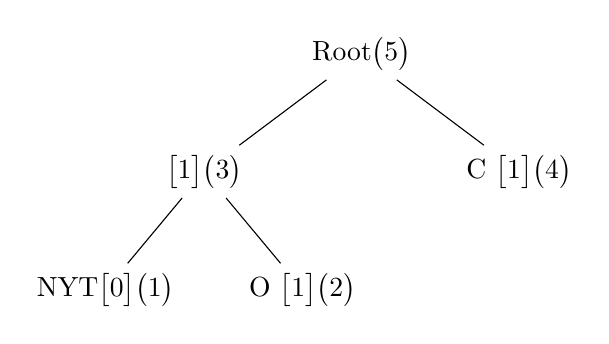
\begin{tikzpicture}[level 1/.style={sibling distance=4cm},level 2/.style={sibling distance=2.5cm},level 3/.style={sibling distance=2cm}]
	\node {Root\big(5\big)}
	    child { node{\big[1\big]\big(3\big)}
	            child { node{NYT\big[0\big]\big(1\big)}}	
		        child { node{O  \big[1\big]\big(2\big)}}}	
		child { node{C  \big[1\big]\big(4\big)}}
	;
\end{tikzpicture} 
\item Code C = 1. Transmit 1. \\
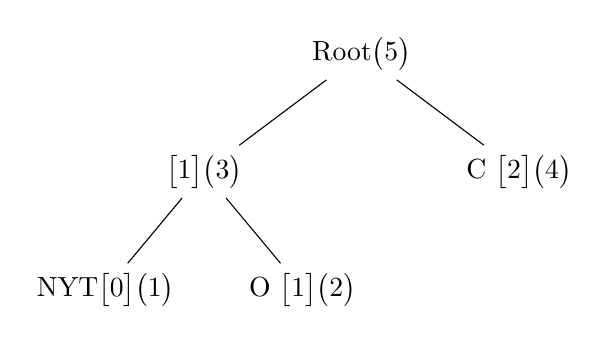
\begin{tikzpicture}[level 1/.style={sibling distance=4cm},level 2/.style={sibling distance=2.5cm},level 3/.style={sibling distance=2cm}]
	\node {Root\big(5\big)}
	    child { node{\big[1\big]\big(3\big)}
	            child { node{NYT\big[0\big]\big(1\big)}}	
		        child { node{O  \big[1\big]\big(2\big)}}}	
		child { node{C  \big[2\big]\big(4\big)}}
	;
\end{tikzpicture}
\item Code O = 01. Transmit 01. \\
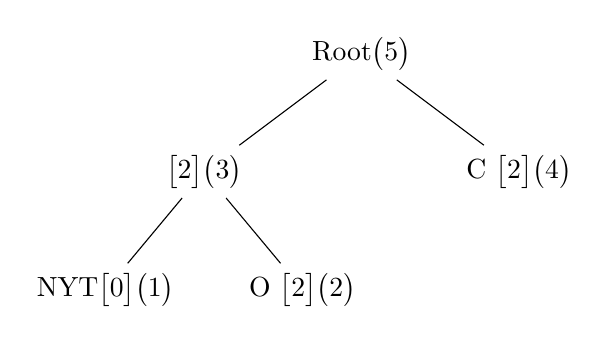
\begin{tikzpicture}[level 1/.style={sibling distance=4cm},level 2/.style={sibling distance=2.5cm},level 3/.style={sibling distance=2cm}]
	\node {Root\big(5\big)}
	    child { node{\big[2\big]\big(3\big)}
	            child { node{NYT\big[0\big]\big(1\big)}}	
		        child { node{O  \big[2\big]\big(2\big)}}}	
		child { node{C  \big[2\big]\big(4\big)}}
	;
\end{tikzpicture}
\item Code A = Code(NYT):Code(A). Transmit 000. \\
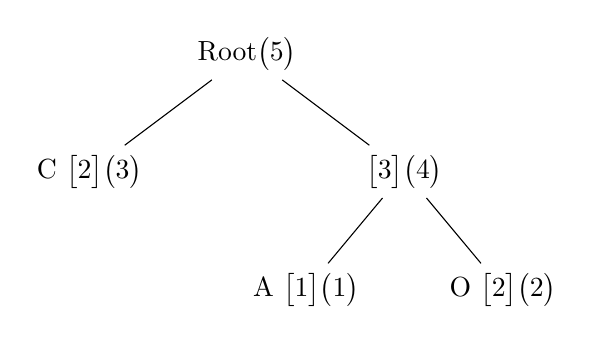
\begin{tikzpicture}[level 1/.style={sibling distance=4cm},level 2/.style={sibling distance=2.5cm},level 3/.style={sibling distance=2cm}]
	\node {Root\big(5\big)}
		child { node{C  \big[2\big]\big(3\big)}}
	    child { node{\big[3\big]\big(4\big)}
	            child { node{A  \big[1\big]\big(1\big)}}	
		        child { node{O  \big[2\big]\big(2\big)}}}	
	;
\end{tikzpicture}
\item Code C = 0. Transmit 0.
\end{itemize}
 $\therefore \text{final code}= 100111010000$
\end{solution}
